\section{RANDBETA Beta Deviate Random Number Generator}

\subsection{Usage}

Creates an array of beta random deviates based on the supplied
two parameters. The general syntax for \verb|randbeta| is 
\begin{verbatim}
   y = randbeta(alpha, beta)
\end{verbatim}
where \verb|alpha| and \verb|beta| are the two parameters of the 
random deviate.  There are three forms for calling \verb|randbeta|.
The first uses two vectors \verb|alpha| and \verb|beta| of the same
size, in which case the output \verb|y| is the same size as both
inputs, and each deviate uses the corresponding values of \verb|alpha|
and \verb|beta| from the arguments.  In the other forms, either
\verb|alpha| or \verb|beta| are scalars.
\subsection{Function Internals}

The probability density function (PDF) of a beta random variable
is
\[
f(x) = x^(a-1) * (1-x)^(b-1) / B(a,b)
\]
for \verb|x| between 0 and 1.  The function \verb|B(a,b)| is defined so
that the integral of \verb|f(x)| is 1.
\subsection{Example}

Here is a plot of the PDF of a beta random variable with \verb|a=3|,
\verb|b=7|.
\begin{verbatim}
--> a = 3; b = 7;
--> x = (0:100)/100; t = x.^(a-1).*(1-x).^(b-1); 
--> t = t/(sum(t)*.01);
--> plot(x,t);
\end{verbatim}
which is plotted as


\centerline{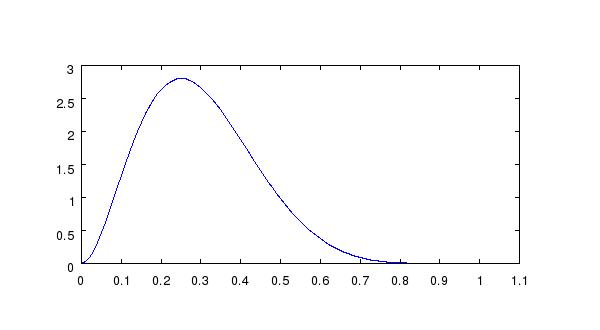
\includegraphics[width=8cm]{betapdf}}

If we generate a few random deviates with these values,
we see they are distributed around the peak of roughly
\verb|0.25|.
\begin{verbatim}
--> randbeta(3*ones(1,5),7*ones(1,5))

ans = 

    0.2777    0.0642    0.3305    0.5259    0.4003 
\end{verbatim}
